% About Unity

\section{External resources}
The Design Review application was implemented by using several pre-made assets.
When the application is started user is positioned into a oiltank model, which was provided by DNV GL. 
This model is of high fidelity and was originally developed for the DNV GL Survey Simulator, an application to train surveyors.

\begin{figure}%[h!] %[H]
	\frame{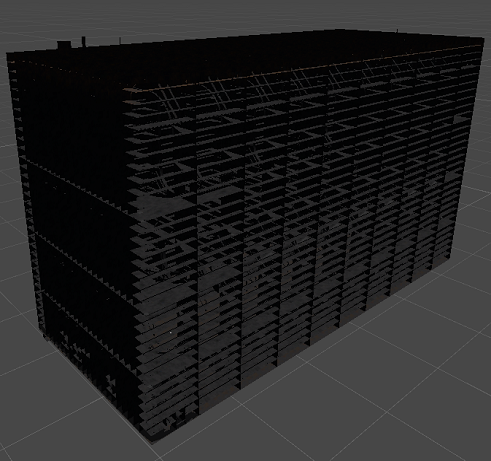
\includegraphics[width=0.5\linewidth]{pictures/tank/back.png}}
	\frame{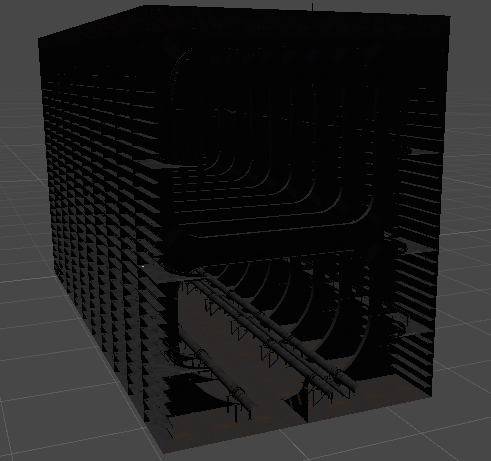
\includegraphics[width=0.5\linewidth]{pictures/tank/half_profile.png}}
	\caption[The Oil tank model]{The Oil tank model from the outside}
	\label{fig:tank_outside}
\end{figure} 

The application also makes use of several "best practice" assets from Leap Motion, Oculus VR and SteamVR to ensure that these devices function
as optimally as possible. From Leap Motion the \texttt{LeapHandController} is utilized, which is a prefab (gameObject), with several important scripts attached to
it. Leap motion provided hand models are also being used, which was provided from the Leap Motion Hands-module. More specifically 
the \texttt{RiggedPepperCutHands} were used, but any other of the hand models could be used as easily.

From Oculus VR two prefabs is used. The first is \texttt{OVRCameraRig}, which is the recommended camera setup for using the Oculus Rift HMD. This 
prefab sets several important settings to ensure that both the head tracking and visual performance is as optimal as possible. The 
second prefab which is used is one called the \texttt{GazePointerRing}. This was showcased in a demo unity implementation by OculusVR
and is essentially a cursor that exist in the game world a fixed length in front of the user. As regular crosshair (which are drawn directly on the screen space)
isn't allowed in VR (more about this later), the \texttt{GazePointerRing} serves as a crosshair. 
From SteamVR the \texttt{[CameraRig]} prefab is used, which essentially does the same configurations as the \texttt{OVRCameraRig} does, but with the HTC Vive HMDs in mind.

The Design review application also makes use of Hover UI Kit, an open source project for creating VR/AR-enabled, customizable and dynamic user interfaces. 
This kit was vital in rapidly prototyping a gesture-enabled menu and a virtual keyboard to the annotation forms.

\section{The architecture}
\begin{figure}%[h!] %[H]
	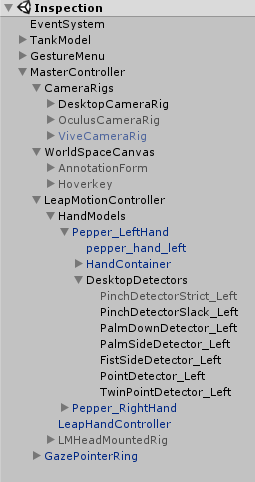
\includegraphics{pictures/unity_hierarchy.png}
	\caption[The Unity project hierarchy of the Design Review Application]{The Unity project hierarchy of the Design Review Application}
	\label{fig:unity_hierarchy}
\end{figure} 

The Unity project has four top-level game objects, as visible in \ref{fig:unity_hierarchy}. 
These will be covered by their own sections, with subsections detailing their important child game objects where appropriate.

% In short terms EventSystem is responsible for processing and handling events and input actions in the scene.
% The TankModel game object contains several child objects that together make up the oiltank-model.
% GestureMenu contains the menu, all its interactable buttons and several scripts.
% The MasterController . 

\section{The master controller}
The \texttt{MasterController} game object represents the player model and contains many of the most important game objects, in addition to
holding many key scripts. The \texttt{MasterController}'s transform, with its position, rotation and scale, represents the user's position and orientation, 
and every child object of \texttt{MasterController} will have a position, rotation and scale that is relative to its own. This ensures
that e.g.~the camera will always "follow" the user. Because this game object is so essential, we will cover several important components and
child objects in the following section.

\begin{figure}%[h!] %[H]
	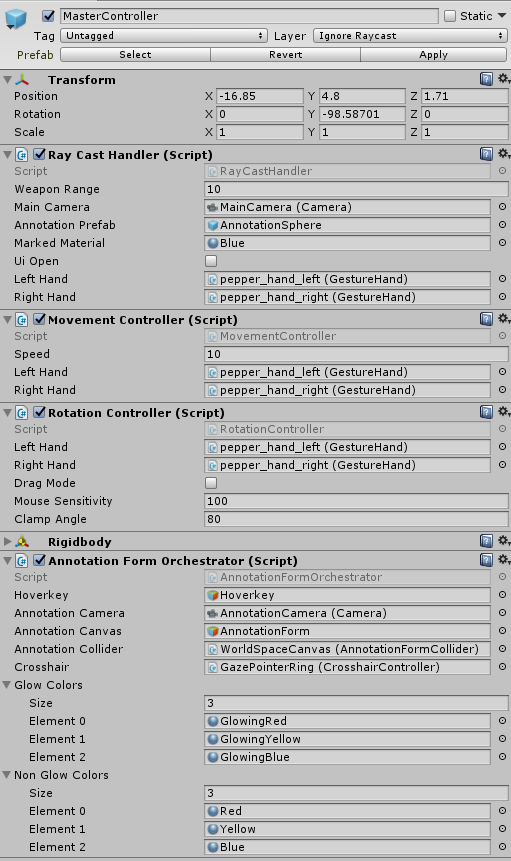
\includegraphics{pictures/unity_inspector.png}
	\caption[The \texttt{MasterController} components]{The \texttt{MasterController} components seen in the Unity Inspector view.}
	\label{fig:unity_inspector}
\end{figure} 

\subsection{The camera rigs}
The \texttt{CameraRigs} game objects holds three different game object, which each represents its own camera-setup: \texttt{DesktopCameraRig}, which is meant to be used
without virtual reality, \texttt{OculusCameraRig}, meant to be used with Oculus Rift HMDs, and \texttt{ViveCameraRigs}, meant to be used with the HTC Vive.
For the application to run successfully one of these rigs should be enabled, while the other two should be disabled.
This can be done by switching between the three rigs in the dropdown-menu named Rig, which is present on the \texttt{CameraRigs} game object itself and
implemented in the \texttt{CameraRigSetup} script. In addition to ensuring that only the correct rig is enabled, 
the \texttt{CameraRigSetup} script also does several other operations. One of these is ensuring that the field of view is set to 60 degrees if the desktop rig 
is selected, as this can wrongfully be set to a HMD's value if a HMD is connected to the computer. When a virtual reality rig is used the field of view is 
set automatically by the HMD software. Another thing done by the script is to decide wheter a two dimensional crosshair/cursor should be drawn on the screen space
(in case of the desktop rig), or if a three dimensional crosshair/cursor (i.e the \texttt{GazePointerRing}) should be drawn in the world space. 

\subsection{The world space canvas}
The \texttt{WorldSpaceCanvas} is a canvas object, which in Unity serves as a container for other user interface elements, such as buttons and input fields, 
and is rendered in world space. It is thus diegetic and exists there like other 3D objects.

In applications that don't utilize virtual reality, canvases and other UI elements are usually non-diegetic (i.e they don't exist within the game world), 
and in 2D and drawn directly to the screen space (as opposed to world space) using x- and y-coordinates.
With this approach one can specify e.g.~a position by its x- and y-coordinate, where \{0, 0\} usually represents the top-left of the display.
This changes in virtual reality applications, as the user's eyes are unable to focus on the screen space. An analogy to this would be to 
ask the user to read a letter while holding it 2-3 centimeters from their eyes. Because of this, elements appearing on the screen space is not rendered
in unity while running it with the virtual reality SDKs. 

\begin{figure}%[h!] %[H]
	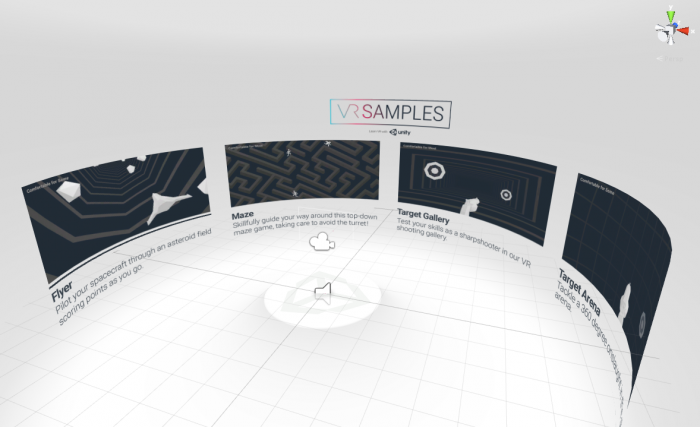
\includegraphics[width=\linewidth]{pictures/unity_vr_menu.png}
	\caption[An example of world-space (diegetic) user interfaces]{An example of world-space (diegetic) user interfaces~\citep{Unity}.}
	\label{fig:unity_vr_menu}
\end{figure} 

Another reason why the canvas is rendered in world space, and also the reason why this is the case in desktop mode, is because of our touch interaction.
To enable the user to click on buttons using his or her hands, the user interface must also exist in world-space so a collision can occur between the desired 
button and the hand models (that mimic the users hand). 

\texttt{WorldSpaceCanvas} is thus rendered in the world space, and is always positioned 0.8 unity meters (i.e the virtual representation of a meter in unity) 
in front of the user. The game object thus always in the center of the camera, but is only visible and enabled when the user is editing an annotation.

\begin{figure}%[h!] %[H]
	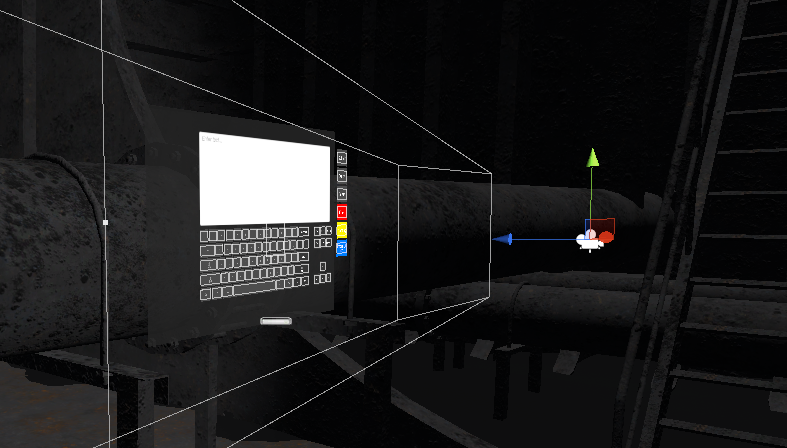
\includegraphics[width=\linewidth]{pictures/tank/worldspacecanvas_scene.png}
	\caption[The \texttt{WorldSpaceCanvas} as seen in the Unity Scene View]{The \texttt{WorldSpaceCanvas} as seen in the Unity Scene View.}
	\label{fig:worldspacecanvas_scene}
\end{figure} 

\begin{figure}%[h!] %[H]
	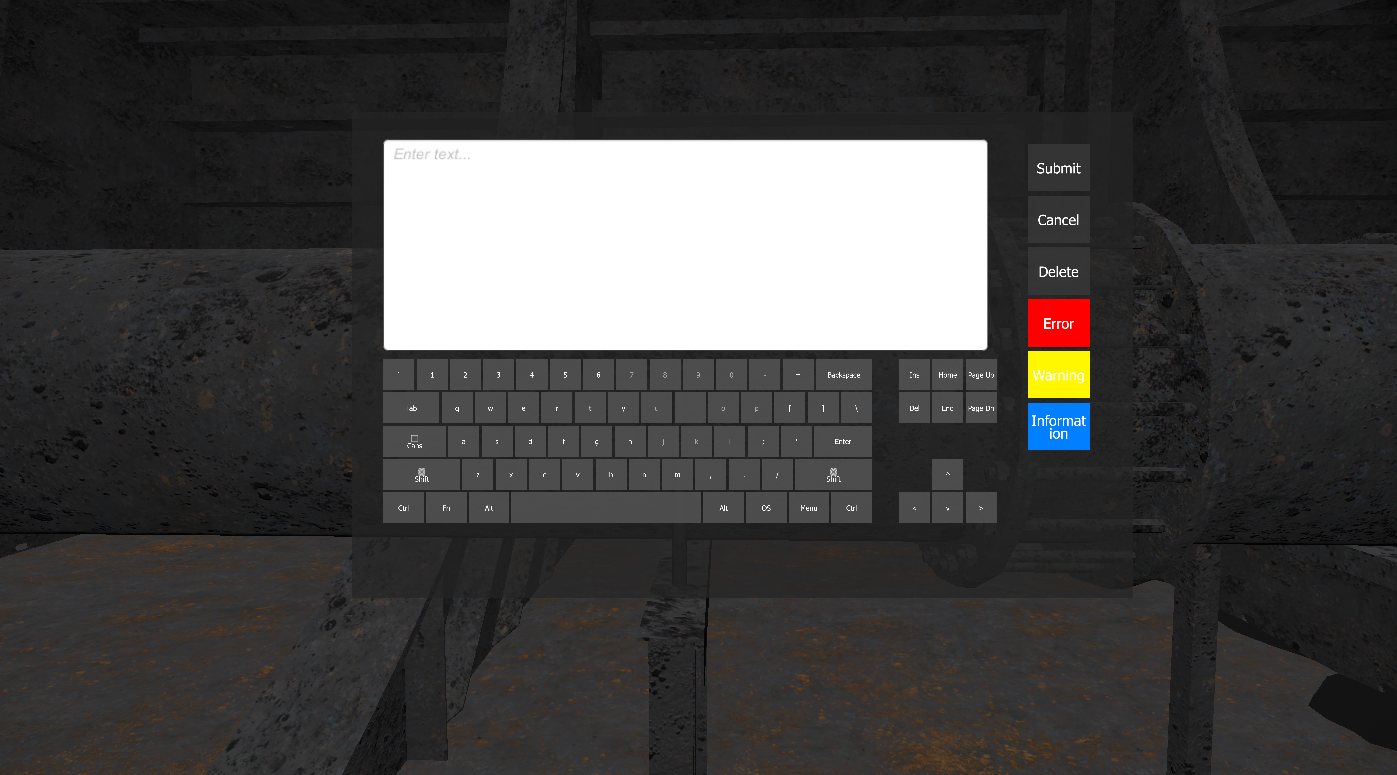
\includegraphics[width=\linewidth]{pictures/tank/worldspacecanvas_ingame.png}
	\caption[The \texttt{WorldSpaceCanvas} as seen in the Unity Game View]{The \texttt{WorldSpaceCanvas} as seen in the Unity Game View.}
	\label{fig:worldspacecanvas_ingame}
\end{figure} 

The \texttt{WorldSpaceCanvas} has two child game objects: \texttt{AnnotationForm} and \texttt{Hoverkey}. 
\texttt{AnnotationForm} currently only contains a inputfield-object and a background rectangle, but can in future iteration grow to 
contain other user interaction elements. The \texttt{Hoverkey} game object represents the touch keyboard and is part of the HoverUI-kit.
In addition to the keyboard six other similar buttons are also present: Submit, Cancel, Delete, Error, Warning and Information (see \ref{fig:worldspacecanvas_ingame}).

\subsection{The Leap Motion Controller}
The \texttt{LeapMotionController} game object contains objects related to the Leap Motion device and gesture recognition and consist primarily of the hand models, necessary 
scrips and detectors. In the game object \texttt{HandModels} there is one object-representation of the left hand, called \texttt{Pepper\_LeftHand}, and one for the 
right hand, called \texttt{Pepper\_RightHand}. These objects have their own hand models (as there needs to be different models for the left and right hand) and their 
own detector objects (as a detector can/should only observe one hand). Each "hand" thus have its own list of detectors called \texttt{Detectors}. 
These are the definition and implementation of the gesture scheme that were discussed in \ref{sec:gesture_design}. As these detectors are a key component of 
this implementation, they will be reviewed in more detail.   
 





% Important child objects of MasterController include CameraRigs, which holds seperate camera rigs for either destop, oculus rift or htc vive usage, 
% WorldSpaceCanvas for drawing user interfaces in the game world, LeapMotionController for aspects related to the Leap Motion and
% GazePointerRing to enable the gazepointer ring when a virtual reality headset is used. These are all documented below.


